\chapter{Analysis and specification of needs}

\noindent Researching the current solutions led us to formulate a set of
requirements to ensure that Merebase offers the best experience.

\section{Functional requirements}

\begin{itemize}
	% \tightlist
	\item
	      A user must signup and login using only their email
	\item
	      A user's account picture is fetched automatically from Gravatar
	\item
	      A user can create a maximum of 20 workspaces \footnote{This is a
		      technical limit imposed by Stripe, the payment processor}
	\item
	      A user can invite other users to their workspace using their email
	\item
	      A user can create new projects, columns, and rows
	\item
	      A user can query the database using a REST endpoint and a Websocket
	      endpoint
	\item
	      A user can upgrade their account to a premium one
	\item
	      A user can cancel their premium subscription
	\item
	      A user can edit the same document as other users at the same time
	\item
	      A user can define the column data type (text, number, boolean, etc.)
\end{itemize}

\section{Non-functional
  requirements}

\begin{itemize}
	% \tightlist
	\item
	      The web app should load within milliseconds
	\item
	      Browsing large documents should not result in glitches or lags
	\item
	      The interface should be accessible and intuitive
	\item
	      Private documents should remain private and inaccessible to hackers
	\item
	      The web app and the real-time server should be always available
\end{itemize}

\section{Identification of actors}

Merebase uses RBAC (Role-Based Access Control) to manage users' access
levels and permissions. There is only one actor, the user, but with
multiple assignable roles.

\begin{itemize}
	% \tightlist
	\item
	      Owner: The user who created the resource, be it the workspace or the
	      project. This role gives you entire access to the resource and it is
	      assigned automatically.
	\item
	      Admin: This role gives non-owner users the same privileges as the
	      owner. Admins can invite new users and assign roles.
	\item
	      Editor: This role permits a user to edit documents in a workspace.
	\item
	      Viewer: This role permits a user to view documents in a workspace,
	      without the ability to modify them.
\end{itemize}

\section{Use case diagrams}

To better illustrate the main interactions between the user and the
application, we rely on a use case diagram.


%\begin{figure}
%\centering
%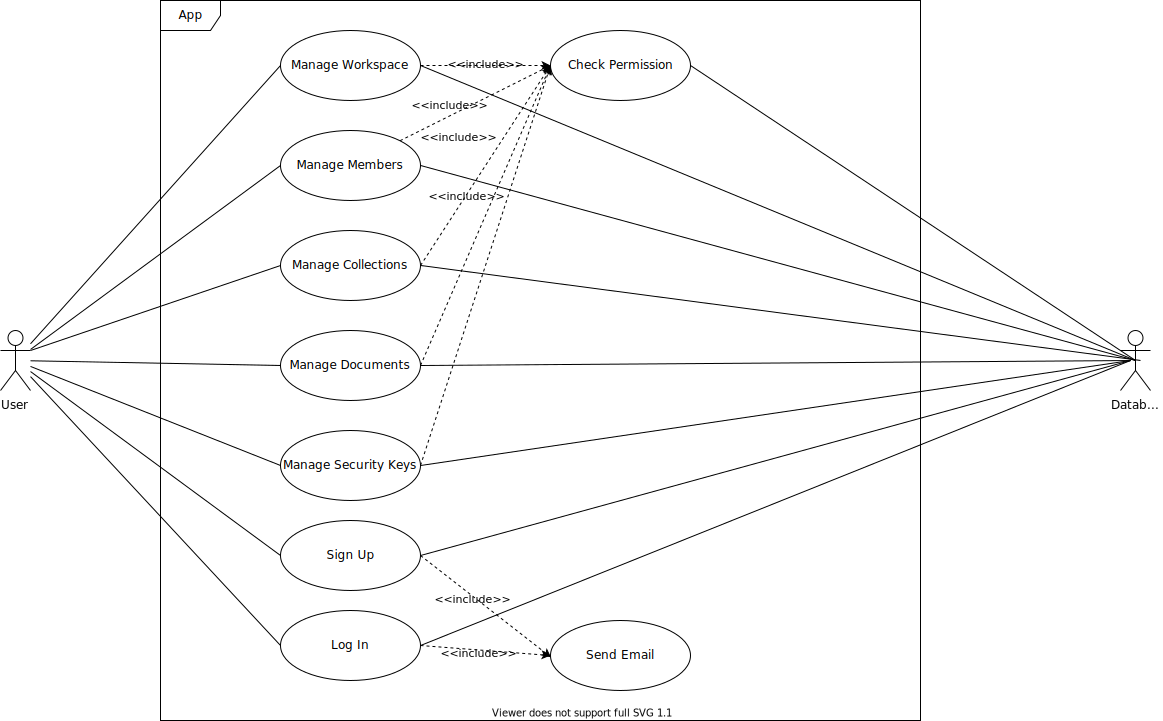
\includegraphics{./assets/UCD, General.svg}
%\caption{General use case diagram}
%\end{figure}

% \begin{tikzpicture}
% 	\draw (0,0) -- (0,4);
% 	\draw (2,2) circle (2);
% \end{tikzpicture}
\begin{figure*}[h]
	\hspace*{-\dimexpr\oddsidemargin+1in\relax}\makebox[\paperwidth]{%
		\begin{tikzpicture}

			\begin{umlsystem}[x=4]{Application}
				\umlusecase{use case 1} % usecase-1
				\umlusecase[y=-2]{use case 2} % usecase-2
				\umlusecase[y=-4]{use case 3} % usecase-3
				\umlusecase[x=4, y=-2, width=1.5cm]{ % usecase-4
					\shortstack{use case 4\\\footnotesize{on 2 lines}}
				}
				\umlusecase[x=6, fill=green!20]{use case 5} % usecase-5
				\umlusecase[x=6, y=-4]{use case 6} % usecase-6
			\end{umlsystem}

			\umlactor{user}
			\umlactor[y=-3]{subuser}
			\umlactor[y=-6]{subsubuser}
			\umlactor[x=14, y=-1.5]{admin}

			\umlinherit{subuser}{user}
			\umlinherit{subsubuser}{subuser}
			\umlassoc{user}{usecase-1}
			\umlassoc{subuser}{usecase-2}
			\umlassoc{subuser}{usecase-3}
			\umlassoc{admin}{usecase-5}
			\umlassoc{admin}{usecase-6}
			\umlinherit{usecase-2}{usecase-1}
			\umlVHextend{usecase-5}{usecase-4}
			\umlinclude[name=incl]{usecase-3}{usecase-4}

			% \umlnote[x=7, y=-7]{incl-1}{
			% 		\footnotesize{note on include dependency}
			% }

		\end{tikzpicture}}

	\caption{Example of a parametric plot ($\sin (x), \cos(x), x$)}

\end{figure*}


\section{Conclusion}

\emph{TBD}